\chapter{BACKGROUND}


Some scholars found that current Boolean search and filtering techniques cannot satisfy the complexity of candidate-job matching requirement.~\cite{malinowski2006matching} They hope the system could understand the job requirement, determine which requirements are mandatory and which are optional but preferable. So they moved to use recommender systems technique to address the problem of information overflow.

There are two main challenges in Content-Based Recommendation Systems: One is how to extract the information from the job descriptions and job seekers' resumes, the other is how to calculate similarity of them.

\section{Job Recommender System}

\subsection{Recommender System}

Job searching is not a new topic in information retrieval, which has been the focus of some commercial job finding web sites and research papers. Usually scholars called them Job Recommender Systems (JRS), because most of them used technologies from recommender systems. Wei et al. classified Recommender Systems into four categories~\cite{wei2007survey}: Collaborative Filtering, Content-based filtering, Knowledge-based and Hybrid approaches. Some of these techniques had been applied into JRS; Zheng et al. ~\cite{siting2012job} and AlOtaibi et al.~\cite{al2012survey} summarized the categories of existing online recruiting platforms and listed the advantages and disadvantages of technical approaches in different JRSs. The categories include:

\begin{enumerate}
    \item Content-based Recommendation (CBR) The principle of a content-based recommendation is to suggest items that have similar content information to the corresponding users, like Prospect \cite{singh2010prospect}.

    \item Collaborative Filtering Recommendation (CFR) Collaborative filtering recommendation, which finds  similar  users  who have  the same taste with the target user and recommends items based on what the similar users, like CASPER~\cite{rafter2000personalised}.

    \item Knowledge-based Recommendation (KBR) In the knowledge-based recommendation, rules and patterns obtained from the functional knowledge of how a specific item  meets the requirement of a particular user, are used for recommending items, like  Proactive~\cite{lee2007fighting}.

\end{enumerate}

\subsection{Job Recommender System}

I will review some existing JRS from some aspects:

\begin{enumerate}
    \item  User information

    \item  Job information

    \item  recommend strategy

\end{enumerate}

Rafter et al. \cite{rafter2000personalised} began to use ACF (Automated Collaborative Filtering) in Job Recommender system, ``CASPER''. In the system user profiles are gotten from server logs, that included: revisit data, read time data, and activity data. All these factors were viewed as measure of relevance among users. The system recommend jobs in two steps. First the system find a set of user related to the target user, second the jobs that related users liked will be recommend to the target user. The system use cluster-based Collaborative Filtering strategy. The similarity between users are based on how many jobs they both reviewed, or applied.

The CASPER also allows user search jobs by a query which is a combination of some fields, like location, salary, and skill etc. The system use such query to find jobs, and the returned jobs will be ranked with above collaborative filtering algorithm.
In their paper, they didn't give a detail description on how to detect the related fields they need and how to the transfer semi-structured job description to structured one. This system is helping job seeker to find jobs.

The shortage of Collaborative Filtering:
 First since the searching result is huge, and the result is sorted randomly, even two very similar users may review different jobs,  or say the probability of two similar users reviewing the same job is low. The authors also noticed the such sparseness problem in users profile, so they try to user cluster-based solution to resolve this problem.

 Second because recommended jobs are from others users searching result, since the current quality of current searching result is low, so the quality of recommendation cannot be high.

F{\"a}rber et al \cite{farber2003automated}. presented a recommender system built on a hybrid approach. The system integrated two methods, content-based filtering and collaborative filtering, and tried to overcome the problem of rating data sparsity by leveraging synergies of a combined model, et. the  latent aspect model. The data they used were synthetic resume. The model they are shown in Figure


\begin{figure}[htbp]
  \centering
  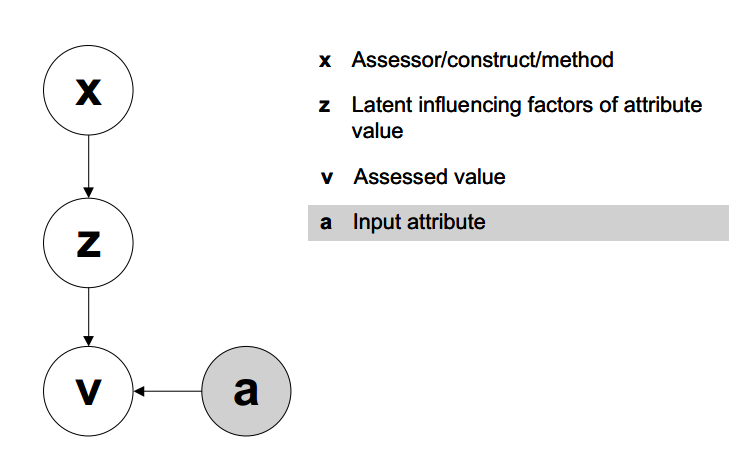
\includegraphics[scale=0.4]{images/la.png}
  \caption{Latent Aspect Model}
  \label{fig:la}
\end{figure}

In Malinowski et al. \cite{malinowski2006matching}, they classified the job recommender systems into two categories,  CV-recommender, which to recommend CVs to recruiter. The job-recommender, which recommend jobs to job seekers.

The system collect the users' profile data by asking input their profiles to the web form based interface field by field. The input data collected are:

\begin{enumerate}
    \item  Demographic data (e.g. date of birth, contact information)

    \item  Educational data (e.g. school courses, grades, university, type of degree, intermediate and final university examinations, postgraduate studies)

    \item  Job experience (e.g. name of the company, type of employment, industry group, occupational field)
    \item  Language skills (e.g. language, level of knowledge)
    \item  IT skills (e.g. type of skill, level of knowledge)
    \item  Awards, scholarships, publications, others   

\end{enumerate}
The system also asked the users upload their resumes, but that's for facilitating the human judgment.

From the paper we know, the model latent aspect model is statistical model, which need to be trained before be applied into recommendation. But training need user to label to data, since current quality of result of job searching is poor, it will take a lot of time for user to train model.  


Drigas* et al.\cite{malinowski2006matching} al presented a expert system to match jobs and job seekers, and recommend unemployed to  The expert system used Neuro-Fuzzy rule to evaluate the matching:
Candidate's X matches X Criterion 
 

The system represent the job in six fields:
\begin{enumerate}
    \item  Age
    \item  Education
    \item  Additional Education(Training) 
    \item  Previous Employment (Experience)
    \item  Foreign Language
    \item  Computer Knowledge
\end{enumerate}

 The system use a relation matrix to represent the fuzzy relation between these specialities. The system need the training data to train that Neuro-fuzzy network. 
 
Both resume data and job info data were manually input into the system  . The fields they selected are relative small.

Daramola et al.  also proposed a fuzzy logic based expert system(FES) tool for online personnel resctuitments. In the paper, the authors assumed that the information already be collected. The system use a fuzzy distance metric to rank candidates' profile in the order of their eligibility for the job. The fuzy hamming distance is given as:
$$ \delta \left ( O,R \right )=\sum_{i=1}^{n}\left | \mu_O(x_i) - \mu_R(x_i)  \right | $$

Ioannis et al. used a machine learned prediction model to recommend new jobs to job seekers.  The features used by the prediction model includes: 

\begin{table}[ht]
\caption{Resume and Job Description} % title of Table
\centering % used for centering table
\begin{tabular}{ l l r }
 \hline
 Feature type &  Feature  &  Range   \\ \hline
              &  company title   & String  \\
Institution   &  industry        & String  \\
              &  company type    & \{public, private\} \\
              &  number of employees &    Num \\  
 \hline  
              &  number of jobs         & Num  \\
              &  position title         & String  \\
  employee    &  best position title    & String \\
              &  years of experience    &    Num \\
              &  number of universities &    Num \\
              &  education degree       & String \\              
 \hline
\end{tabular}
\label{tab:predictionmodel} % is used to refer this table in the text
\end{table}

\begin{table}[ht]
\caption{Comparison of Job Recommender Systems } % title of Table
\centering % used for centering table
\begin{tabular}{ | c |  p{6cm} | p{6cm} | } % centered columns (4 columns)

\hline  %inserts double horizontal lines
 System & Approach  & User Information  \\ [0.5ex] % inserts table
%heading
\hline % inserts single horizontal line
 &
    \begin{singlespace}
       \textbullet~Declarative  \par
       \textbullet~Easy to comprehend  \par
       \textbullet~Easy to maintain\par
       \textbullet~Easy to incorporate domain knowledge\par
       \textbullet~Easy to trace and fix the cause of errors  \par
    \end{singlespace}
    &  \begin{singlespace}
      \textbullet~Heuristic \par
       \textbullet~Requires tedious manual labor \par
       \end{singlespace}  \\
\hline
ML-based &
    \begin{singlespace}
       \textbullet~Trainable  \par
       \textbullet~Adaptable \par
       \textbullet~Reduces manual effort \par
    \end{singlespace}
    &  \begin{singlespace}
      \textbullet~Requires labeled data \par
       \textbullet~Requires retraining  for domain adaptation \par
        \textbullet~Requires ML expertise  to use or maintain \par
       \textbullet~Opaque  \par
       \end{singlespace} \\
\hline %inserts single line
\end{tabular}
\label{tab:jrcom} % is used to refer this table in the text
\end{table}




\section{Information Extraction}
One important the problem of this system is how to build the models from Job Description and Resume. The first step of model generating is information extraction. Both resumes and job descriptions are written in natural language, so we need to extract information from such un-structured or semi-structured data source, and transfer them to some designed structure.

\subsection{Machine learning and Rule-based IE technologies}

Chiticariu et al. \cite{chiticariu2013rule}summarized the pros and cons of machine learning (ML) and rule-based IE technologies in Table

\begin{table}[ht]
\caption{Pros and Cons of ML and Rule-Based IE technologies } % title of Table
\centering % used for centering table
\begin{tabular}{ | c |  p{6cm} | p{6cm} | } % centered columns (4 columns)

\hline  %inserts double horizontal lines
 & Pros  & Cons  \\ [0.5ex] % inserts table
%heading
\hline % inserts single horizontal line
Rule-based &
    \begin{singlespace}
       \textbullet~Declarative  \par
       \textbullet~Easy to comprehend  \par
       \textbullet~Easy to maintain\par
       \textbullet~Easy to incorporate domain knowledge\par
       \textbullet~Easy to trace and fix the cause of errors  \par
    \end{singlespace}
    &  \begin{singlespace}
      \textbullet~Heuristic \par
       \textbullet~Requires tedious manual labor \par
       \end{singlespace}  \\
\hline
ML-based &
    \begin{singlespace}
       \textbullet~Trainable  \par
       \textbullet~Adaptable \par
       \textbullet~Reduces manual effort \par
    \end{singlespace}
    &  \begin{singlespace}
      \textbullet~Requires labeled data \par
       \textbullet~Requires retraining  for domain adaptation \par
        \textbullet~Requires ML expertise  to use or maintain \par
       \textbullet~Opaque  \par
       \end{singlespace} \\
\hline %inserts single line
\end{tabular}
\label{tab:mlrb} % is used to refer this table in the text
\end{table}

Yu et al.~\cite{yu2005resume} used a cascaded information extraction (IE) framework to get the detailed information from the job seeker��s resume. In the first stage, the Hidden Markov Modeling (HMM) model is used to segment the resume into consecutive blocks. Based on the result, a SVM model is used to obtain the detailed information in the certain block, the information include: name, address, education etc.

 Celik Duygua and Elci Atilla proposed a Ontology-based R��sum�� Parser (ORP) ~\cite{ccelik2013ontology}, which uses ontology to assistant the information extraction process. The system process the resume in following steps: convert the resume files into plain text, separate the text into  some segments, use Ontology Knowledge Base to find the concepts in the sentences, normalize all the terms, at last the system will classify the sentences to get the wanted terms.

\section{Matching Algorithms}

Lu et al~\cite{lu2013recommender}. used latent Semantic Analysis(LSA) to calculate similarities between jobs and candidates, but they only selected two factors ``interest'' and ``education''  to compare candidates. Xing et al. ~\cite{yi2007matching} used Structured Relevance Models (SRM) to  match resumes and jobs.

The Ontology technics had also been used in some JRSs, which had been well studied by  Shvaiko and Euzenat in \cite{shvaiko2013ontology}.  Proactive~\cite{lee2007fighting} used two kinds of ontology, job category and the company information. The system used ontology checker to classify the job information, stored the domain knowledge and calculated the weight value in recommendations.

Kumaran et al~\cite{kumaran2013towards} also used ontology to calculate the similarity between job criteria and candidates's resume in their system~\cite{kumaran2013towards}. The similarity equation they used are:
$$ M\left ( i_1, i_2 \right ) = \frac{\sum_{k=1}^{n} Sim\left (p_{k}^{i1},  p_{k}^{i2} \right ) * W_{k}^{i2}}{\sum_{k=1}^{n} W_{k}^{i2}}  $$
The similarity function $Sim(p_1, p_2)$ is defined as follows:
$$ Sim(p1, p2) = \begin{Bmatrix}
1, & if~similarity~of~p1~and~p2 \geqslant t\\
0, & otherwise
\end{Bmatrix} $$

Fazel \cite{fazel2009semantic} used a hybrid approach to matching job seekers and job postings, which takes advantage of the benefits of both logic-based and ontology-based matching. In his paper the description logics (DL) is used to represent the candidate and job opening, and the ontology is used to organize the skills in a skill taxonomy. He gave an equation to calculate the matching degree:
$$ sim\left(P ,j \right) = \sum x_{ij} \times u(ds_i) $$

where, $x_{ji}$ is the Boolean variable indicating whether desire i is satisfied by applicant $A_{j}$ in the set of all qualified applications.

Liu and Dew~\cite{liu2004using} used RDF to represent and store the expertise of experts , and a RDF-based Expertise Matcher could retrieves the experts whose expertise include the required concept.
